%File: formatting-instruction.tex
\documentclass[letterpaper]{article}
\usepackage{flairs}%aaai
\usepackage{times}
\usepackage{helvet}
\usepackage{courier}
%\usepackage{url}
\usepackage[hyphens]{url}
\usepackage{hyperref}
% for figure grid
\usepackage{graphicx}
\graphicspath{ {figures/} }
\usepackage{caption}
\usepackage{subcaption}
\usepackage{wrapfig}
\usepackage{multirow}
\usepackage{tabularx}
\usepackage{paralist}
\usepackage{colortbl}
\usepackage{dingbat, pifont}
\usepackage{listings}
\usepackage[T1]{fontenc}

\lstset{
  basicstyle=\ttfamily\small,
  columns=fullflexible,
  breaklines=true,
  frame=single,
  captionpos=b
}
\definecolor{Gray}{gray}{0.9}

\usepackage{array} %for table fix width

\frenchspacing
\setlength{\pdfpagewidth}{8.5in}
\setlength{\pdfpageheight}{11in}
\pdfinfo{
/Title (Towards Deterministic Sub-0.5 µs Response on Linux through Interrupt Isolation)
/Author (Anonymous)}
\setcounter{secnumdepth}{0}  

\begin{document}
% This file is an adoption of the style file for AAAI Press 
% proceedings, working notes, and technical reports.  This file is made 
% with minimal changes by explicit permission from AAAI.
%
\title{Towards Deterministic Sub-0.5 µs Response on Linux through Interrupt Isolation}
\author{
\begin{tabular}{lllll}
  Zhouyi Zhou & Zhili Liu & Shancong Zhang & Jiemin Li & Dengke Du \\
 %  & Dengke Du & Mengke Sun  & Zhiqiang Wang & Hongyan Liu & Guoxin Xu & Yexin Han\\
\end{tabular}
\\
Beijing Ucas Technology Co,Ltd., Beijing, China\\
\{zhouyi.zhou, zhili.liu, sam.zhang, jiemin.li,
dengke.du\}@ucas.com.cn\\ 
}

\maketitle

\begin{abstract}
Real-time responsiveness in Linux is often constrained by interrupt contention and timer
handling overhead, making it challenging to achieve sub-microsecond latency.
This work introduces an interrupt isolation approach that centralizes and minimizes timer
interrupt interference across CPU cores. By redirecting periodic timer events to a
dedicated core and suppressing redundant inter-processor interrupts, our design significantly
reduces jitter and response latency. Experiments conducted on an ARM-based multicore
platform demonstrate that the proposed mechanism consistently achieves sub-0.5 µs response
times, outperforming conventional Linux PREEMPT-RT configurations. These results highlight
the potential of interrupt isolation as a lightweight and effective strategy for
deterministic real-time workloads in general-purpose operating systems.
\end{abstract}

\section{Introduction}

Modern high-performance and real-time systems increasingly demand 
\textbf{predictable CPU behavior}, \textbf{ultra-low interrupt latency}, 
and \textbf{minimal system noise}. 
However, general-purpose operating systems such as Linux were not 
originally designed to meet such stringent timing requirements. 
As a result, applications with tight latency constraints often suffer from 
\textbf{execution disturbances} caused primarily by two kernel-level 
mechanisms: \emph{periodic timer interrupts} and 
\emph{inter-processor interrupts (IPIs)}.  

\subsection{Timer Interrupts}
In Linux, periodic timer interrupts (commonly referred to as \emph{ticks}) 
are scheduled on every CPU core to maintain system time and perform 
kernel housekeeping tasks. These interrupts invoke routines for 
timekeeping, task scheduling, timer expiration, bandwidth enforcement 
for real-time processes, and other internal kernel mechanisms. 
While harmless---or even beneficial---for general workloads, 
such periodic processing can be highly disruptive for 
latency-sensitive applications such as user-space packet processing, 
real-time control loops, and multimedia pipelines, where 
\textbf{deterministic CPU execution} is critical.  

Mechanisms such as \texttt{NOHZ\_FULL} attempt to mitigate this problem 
by reducing tick frequency, but they cannot fully eliminate timer activity. 
Even in \texttt{nohz\_full} mode, periodic ticks still occur, leaving 
``isolated'' cores subject to residual interruptions.  

\subsection{Inter-Processor Interrupts (IPIs)}
In addition to timer ticks, IPIs represent another significant source of 
jitter. Within the Linux kernel, IPIs are widely used to coordinate state 
changes across cores---for example, to initiate TLB shootdowns, 
wake remote tasks, or synchronize RCU grace periods. 
From the perspective of an application pinned to a dedicated core, 
IPIs are asynchronous and unpredictable, often leading to unwanted 
preemptions or context switches.  

Disabling local timer interrupts reduces some noise but does not prevent 
a core from receiving IPIs initiated elsewhere in the system. 
Consequently, even cores exempt from ticks may still face arbitrary 
interruptions caused by global kernel coordination mechanisms.  

\subsection{Motivation}
These limitations highlight a fundamental challenge: 
\textbf{conventional mechanisms are insufficient for achieving 
sub-microsecond, deterministic response times in Linux}. 
To address this, we propose an \textbf{interrupt isolation framework} 
that centralizes timer interrupt handling and suppresses unnecessary IPIs, 
thereby enabling Linux systems to deliver 
\textbf{sub-0.5~$\mu$s response times} for real-time workloads.  

\subsection{Our Approach: Full Isolation via Centralized Timer Handling and Shared-Memory IPI Management}

In this paper, we present a novel and more aggressive approach to CPU isolation in Linux, 
designed to achieve deterministic sub-microsecond response times. 
Our mechanism introduces two key innovations:

\begin{itemize}
    \item \textbf{Centralized Timer Handling:} Timer interrupt processing is completely disabled on selected cores. 
    All kernel tick-related activities are redirected to a dedicated maintenance core, 
    which periodically executes the timer functionalities required for global correctness. 
    This ensures that isolated cores run without local timer interruptions.
    
    \item \textbf{Shared-Memory IPI Management:} Non-essential inter-processor interrupts (IPIs) to isolated cores 
    are suppressed. Coordination that would normally trigger IPIs is instead implemented via shared memory, 
    allowing controlled and predictable communication without asynchronous preemption.
\end{itemize}

This level of isolation is not achievable with existing mechanisms such as 
\texttt{NOHZ\_FULL} or \texttt{isolcpus} alone. 
By explicitly separating time-related kernel responsibilities and reassigning them to a dedicated core, 
and by handling inter-core coordination through shared memory rather than IPIs, 
isolated cores execute continuously without interruption.  

The proposed approach is particularly effective in latency-critical scenarios, 
such as GPIO toggling, real-time control loops, and user-space packet processing. 
It allows the Linux kernel to efficiently manage global interrupts, 
isolate real-time workloads on dedicated cores, and guarantee timely execution 
of high-precision tasks free from interference by timer events or other system operations.

\section{Related Work}\label{BG}
\subsection{Timer Interrupt Control in the Linux Kernel}

The concept of timer tickers in operating systems predates the development of the Linux kernel \cite{Corbet}. 
In Linux, periodic timer interrupts, commonly referred to as \emph{ticks}, are scheduled on each CPU core 
to support timekeeping, process accounting, and scheduler activation. These interrupts typically occur at 
frequencies between 250 Hz and 1 kHz and may preempt running tasks to perform kernel maintenance.  

To reduce the overhead caused by frequent ticks, \emph{tickless} systems were introduced. 
The \texttt{NO\_HZ} feature disables timer interrupts on idle CPUs, and its extension, 
\texttt{NOHZ\_FULL}, attempts to eliminate ticks even during active user-space execution \cite{KernelDocNOHZ}. 
However, timer ticks still occur on \texttt{NO\_HZ}/\texttt{NOHZ\_FULL} CPUs because the kernel must perform 
statistics collection and other internal bookkeeping \cite{stackoverflow}.  

While these mechanisms help reduce timer-induced jitter, they do not completely eliminate all sources of latency, 
leaving real-time workloads exposed to residual interruptions.


\subsection{Inter-Processor Interrupts (IPIs) and Their Effects}

Inter-processor interrupts (IPIs) in Linux can significantly impact real-time performance by introducing 
unpredictable latency. IPIs force a CPU to handle interrupts originating from another processor, 
potentially preempting time-critical tasks. In real-time systems, where deterministic scheduling and 
minimal latency are essential, IPIs—used for operations such as TLB flushes, cache management, 
and scheduler balancing—can cause delays if triggered during the execution of high-priority tasks. 
Unlike timer interrupts, IPIs are externally triggered and often asynchronous. Consequently, even 
tickless CPUs may receive unexpected IPIs, introducing nondeterministic latency and potential cache 
disruptions. Existing research has identified IPIs as a major obstacle to achieving strict real-time 
performance on Linux \cite{YuxinRen}.  

To mitigate the impact of IPIs on real-time workloads, it is necessary to systematically identify and 
address each source of cross-core interrupts. For example, unloading block devices in Linux triggers 
IPIs, so such operations should be avoided in latency-critical environments. Similarly, CPU frequency 
statistics require IPIs to query other cores; disabling dynamic frequency scaling or using a fixed-frequency 
mode eliminates this source of latency. By analyzing and selectively suppressing IPI-inducing operations—such as 
TLB shootdowns, RCU callbacks, and scheduler balancing—we can remove unnecessary cross-core interruptions, 
ensuring deterministic execution for real-time tasks. Combined with CPU isolation and IRQ affinity tuning, 
this targeted approach helps maintain hard real-time guarantees on Linux systems.



\subsection{CPU Isolation Techniques}

Linux provides mechanisms such as \texttt{isolcpus} and IRQ affinity \cite{KernelDocParam} 
to isolate processor cores from the general scheduler and external interrupts. 
These tools can effectively prevent a core from executing most kernel tasks and services, 
including RCU callbacks. However, they do not block all types of interruptions. 
In particular, timer interrupts and inter-processor interrupts (IPIs) may still be delivered 
to an isolated core. Consequently, while \texttt{isolcpus} and IRQ affinity reduce interference 
from the operating system, they do not achieve complete isolation at the hardware interrupt level.  

Redhawk Linux RTOS \cite{redhawk} further minimizes the impact of clock interrupts on real-time workloads 
through specialized kernel modifications. These mechanisms significantly reduce the influence 
of inter-core interrupts on system performance. Nonetheless, Redhawk does not entirely eliminate 
inter-core interrupts on isolated cores; instead, they may still occur conditionally under certain scenarios.


\section{Methodology}\label{BE}

This section describes the kernel-level design, isolation strategy, and implementation workflow we employed
to eliminate system noise on real-time application cores without delegating maintenance tasks to external
housekeeping cores. In contrast to traditional separation approaches, our system uses a novel method
where the application core invokes clock maintenance functions on demand via a centralized interface.
This design is made possible through the custom Isolator API v0.1, which we developed to enable complete
tick and IPI suppression while preserving system functionality through cooperative execution.

\subsection{System Design Overview}
\label{subsec:system-design}

The system architecture is designed to provide a robust, low-latency environment for real-time applications by leveraging the concept of core isolation. The central premise is to dedicate one or more processor cores to run real-time tasks exclusively, shielding them from non-deterministic interference from the general-purpose operating system (OS), specifically Linux. This is achieved through a managed isolation lifecycle that suppresses OS services and then reintroduces them in a controlled manner for necessary maintenance.

The design, illustrated in Figure~\ref{fig:isolator_flow}, is built around three core mechanisms:

\begin{enumerate}
    \item \textbf{Isolation Enabling:} The process begins by invoking \texttt{isolator\_start()} with a specified mask (e.g., \texttt{ISOLATOR\_MASK\_CLOCK}, \texttt{ISOLATOR\_MASK\_RESCHED}, \texttt{ISOLATOR\_MASK\_IPI}). This function initiates the isolation state on a core, effectively severing its interaction with standard OS interrupt mechanisms. Crucially, this involves suppressing Inter-Processor Interrupts (IPIs) by replacing them with a deterministic, shared-memory-based message-passing system for cross-kernel communication. It also halts Linux's periodic timers, such as the scheduler tick and real-time bandwidth timer, to prevent any OS-induced preemption or processing during the critical real-time execution window.

    \item \textbf{Periodic Maintenance via a Ticker:} While isolated, the core executes its real-time workload without interruption. However, to maintain system health and coherence, certain clock-related functions must still be performed periodically or on-demand. This is handled by the \texttt{isolator\_tickor()} function, which is invoked by the application itself. This function acts as a managed tick, allowing the isolated core to voluntarily execute maintenance tasks---such as scheduling decisions (\texttt{TICKER\_SCHED}), real-time task management (\texttt{TICKER\_RT}), and time synchronization (\texttt{TICKER\_TSC\_SYNC})---at a time of its choosing, thus preserving determinism.

    \item \textbf{Isolation Teardown:} Upon completion of the real-time task, the isolation state is ended. This final stage gracefully reintegrates the core back into the broader OS environment. The mechanism restarts the standard Linux periodic timers and re-enables the full IPI handling, ensuring the core returns to normal operation without any residual state from the isolation period.
\end{enumerate}

In summary, the design replaces the traditional preemptive, interrupt-driven OS model on isolated cores with a self-managed, cooperative paradigm. The real-time application retains full control over when and how maintenance occurs, resulting in significantly improved timing predictability and performance for latency-sensitive workloads.

\begin{figure}[htbp]
    \centering
    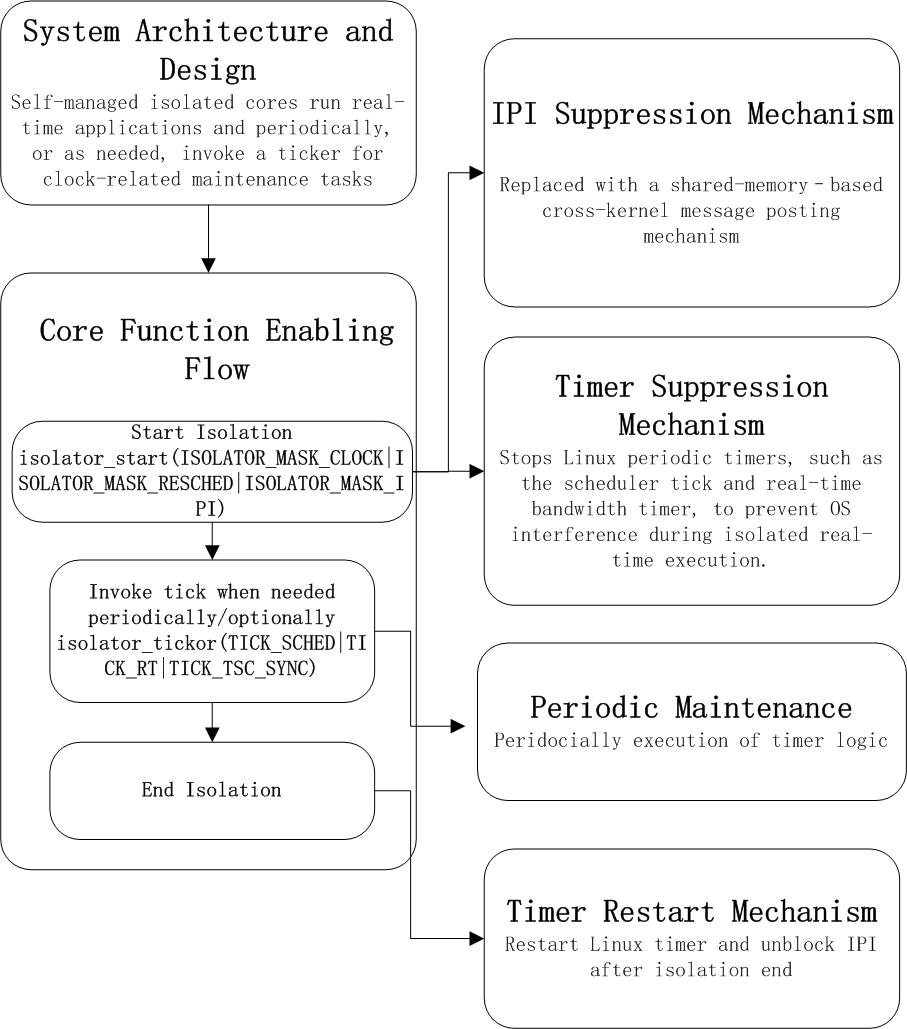
\includegraphics[width=0.9\linewidth]{Isolator.jpg}
    \caption{Core isolation enabling flow and mechanisms.}
    \label{fig:isolator_flow}
\end{figure}


\subsection{Interrupt Suppression and Timer Bypass}
\label{subsec:interrupt-timer}

The kernel was modified to explicitly recognize the isolation state of a core.
When a core is set to isolation mode, its local tick logic, normally executed in
\texttt{update\_process\_times} and \texttt{scheduler\_tick},
is completely bypassed unless explicitly triggered through the \texttt{isolator\_tickor} function.
In addition, all asynchronous inter-processor interrupts (IPIs) that might interfere with the
isolated core are suppressed. The key mechanisms implemented for timer bypass and interrupt suppression are described below.

\paragraph{Timer Suppression}  
The \texttt{isolator\_start} function halts Linux’s periodic tick timer by calling \texttt{hrtimer\_cancel} to
prevent interference from the operating system. In addition, real-time bandwidth timers are maintained in a list,
and each active timer is iteratively canceled to stop any scheduled callbacks. As a result, both the scheduler tick
and other periodic kernel activities on the isolated core are effectively stopped.

\paragraph{IPI Suppression and Replacement}  
Asynchronous IPIs, which are normally used for inter-core notifications, are replaced with a deterministic,
shared-memory-based message posting mechanism. This enables controlled core-to-core communication without
the unpredictability of standard IPIs. Specific handling includes:
\begin{itemize}
    \item \textbf{RCU (Read-Copy Update):} Upon entering isolation, the RCU subsystem is notified that the core is isolated and must be excluded from grace period calculations. 
    \item \textbf{TLB Shootdowns:} IPIs requesting Translation Lookaside Buffer flushes are suppressed and queued in shared memory.
      The isolated core processes these flush requests the next time it invokes \texttt{isolator\_tickor}.
    \item \textbf{CPU Frequency Scaling:} IPIs induced by CPU frequency changes are disabled to avoid unwanted interruptions.
\end{itemize}

\paragraph{Timekeeping}  
Even after stopping periodic timers, the isolated core maintains a consistent notion of system time through \texttt{isolator\_get\_monotonic\_time}, which provides a linearized timestamp in microseconds. The \texttt{isolator\_poll\_until} function allows predictable wake-ups for polling operations without relying on standard kernel timers.

\paragraph{Periodic Maintenance}  
Deferred timer tasks and queued IPI processing are executed only when the isolated core voluntarily calls \texttt{isolator\_tickor}. This ensures deterministic behavior while still allowing the core to perform necessary maintenance tasks at controlled intervals.

\paragraph{Restoration Mechanism}  
When isolation ends, previously canceled Linux timers and real-time bandwidth timers are restarted, and normal IPI handling is restored. The core then returns to standard operation, with all periodic activities and inter-core notifications resumed.


\subsection{Memory and Communication Management}
\label{subsec:memory-communication}

Memory operations required during isolation are handled using a dedicated SLUB allocator reserved for the isolated core. All allocations and deallocations occur within this core-specific SLUB, and cross-core memory maintenance or access is strictly prohibited. This ensures that memory operations remain deterministic and fully isolated from other cores, avoiding interference from general-purpose kernel allocators.

For core-to-core interactions, a shared-memory-based messaging mechanism is employed to transfer messages between the isolated core and non-isolated cores. This mechanism eliminates the need for interrupts to wake remote threads, preserving the deterministic behavior of the isolated core. The primary communication methods are \texttt{post} and \texttt{poll}. Messages intended for a remote core are written into a shared memory region using \texttt{post}, while the receiving core periodically checks for new messages using \texttt{poll}. Callback functions can be registered to handle incoming messages in a non-intrusive, user-driven manner. This design guarantees that all communication occurs without generating asynchronous interrupts, allowing the isolated core to exchange information safely while maintaining strict determinism.

\subsection{Isolation Monitoring and Debugging}
\label{subsec:isolation-monitoring}

To support verification and monitoring of isolated cores, we implemented a real-time statistics collector. This collector tracks the types and counts of interrupts that are blocked or deferred on each core. By analyzing these statistics, developers can verify the effectiveness of the isolation mechanisms and assess the impact of different workloads and tuning configurations. This monitoring infrastructure provides a clear view of the core’s behavior under isolation, enabling precise debugging and performance evaluation.

\section{Implementation Details}
This section presents a detailed overview of the kernel-level modifications we introduced to
support high-determinism, low-jitter execution on isolated CPUs for high-performance, real-time
packet processing. These modifications are implemented within four critical subsystems of the
Linux kernel: RCU (Read-Copy-Update), the Real-Time Scheduler, SMP/IPI handling, and Timer Tick
Management. 

\subsection{Kernel Modifications Overview}
To enable CPU isolation at a fine granularity and ensure minimal OS interference on application-
dedicated cores, we performed targeted changes across the kernel. The key goals are to:
Eliminate unnecessary kernel activity on isolated CPUs,
Avoid inter-processor communication (e.g., IPIs) to reduce latency spikes,
Defer time-based maintenance (e.g., scheduling enforcement) to application-controlled contexts,
To coordinate the behavior of different kernel components, we define the following per-CPU data
structure:

\begin{lstlisting}[language=C, caption={Per-CPU isolator counter definition}]
DEFINE_PER_CPU(atomic_t,
    isolator_counters[CONFIG_NR_CPUS]);
\end{lstlisting}
Each entry in this array acts as a flag indicating whether the corresponding CPU is currently under
isolation. This flag is incremented by user-space applications via a custom system call or API
(isolator\_start()) and is read by kernel components to selectively disable or defer their operations.


\subsection{RCU Grace Period Handling}
This modification ensures that CPUs marked as isolated are treated as being in a permanent
quiescent state by the RCU subsystem. By doing so, the system avoids unnecessary waiting on
isolated cores during RCU grace periods. This approach maintains forward progress of the RCU
mechanism while eliminating dependencies on cores that are no longer expected to participate in
normal kernel activity.

Such treatment is especially crucial in real-time and low-latency systems where isolated CPUs are
fully dedicated to user-level workloads and should not incur involuntary kernel participation.
We add following following condition to kernel function rcu\_implicit\_dynticks\_qs:
\begin{lstlisting}[language=C, caption={Forcing quiescent state if isolator counter is active}]
if (isolator_counters[rdp->cpu].counter) {
    return 1; // Force quiescent state
}
\end{lstlisting}
Another important technical detail is that we explicitly prevent the \texttt{rcu\_preempt} kernel 
thread from running on isolated CPUs. During our experiments, we observed that the scheduler 
occasionally places the \texttt{rcu\_preempt} kernel thread on an isolated core. Since these cores 
are typically occupied by uninterrupted, high-priority user tasks, the \texttt{rcu\_preempt} 
thread may not get scheduled in a timely manner. This situation blocks the progress of RCU grace 
periods, preventing \texttt{synchronize\_rcu} from returning, which in turn causes other processes 
invoking \texttt{synchronize\_rcu} to remain blocked. By disallowing \texttt{rcu\_preempt} on 
isolated CPUs, we avoid this pathological scenario and preserve the expected non-blocking behavior 
of RCU for the rest of the system.  

\subsection{Time Scheduler Deferral}
\paragraph{Tick Subsystem Modifications.}
The Linux \texttt{tick-sched.c} subsystem manages periodic scheduling ticks and 
nohz (tickless) operation. By default, each CPU receives periodic tick events 
driven by high-resolution timers, which are used to drive process accounting, 
timekeeping, and load balancing. However, on isolated CPUs dedicated to 
real-time packet processing, these periodic ticks represent an unnecessary 
source of nondeterministic interruptions.

To address this, we introduced a per-CPU flag (\texttt{ucas\_counter}) that 
controls whether tick-related hrtimers should be restarted or suppressed. When 
this counter is non-zero, functions such as \texttt{tick\_nohz\_restart()}, 
\texttt{tick\_nohz\_idle\_restart\_tick()}, \texttt{tick\_nohz\_handler()}, 
and \texttt{tick\_sched\_timer()} are modified to immediately return without 
restarting the periodic scheduler timer. This effectively disables the 
recurring tick on isolated CPUs, preventing spurious wakeups and involuntary 
kernel execution.

In order to preserve correctness, we provide helper routines that allow the 
isolator subsystem to explicitly handle deferred tick events when needed. For 
example, the function \texttt{ucas\_handle\_tick\_sched\_timer()} invokes 
\texttt{tick\_sched\_do\_timer()} and \texttt{update\_process\_times()} 
manually, ensuring that accounting and timekeeping can still progress under 
controlled conditions.

We also provide utility functions such as 
\texttt{ucas\_stop\_sched\_timer()} to explicitly cancel tick timers when 
isolation is active. 
\begin{lstlisting}[language=C, caption={Stop per-CPU scheduler timer}]
void ucas_stop_sched_timer(void)
{
    struct tick_sched *ts = this_cpu_ptr(&tick_cpu_sched);
    hrtimer_cancel(&ts->sched_timer);
}
\end{lstlisting}

This design guarantees that isolated CPUs are free from involuntary tick 
interrupts during real-time workloads, while still allowing deferred handling 
of system housekeeping activities when explicitly triggered. The result is a 
significant reduction in jitter and improved determinism for 
latency-sensitive applications.

\paragraph{Real-Time Bandwidth Deferral.}
In addition to suppressing periodic tick timers, we extended the real-time (RT) 
scheduler’s bandwidth control logic in \texttt{kernel/sched/rt.c}. In the 
unmodified kernel, each CPU uses a periodic high-resolution timer 
(\texttt{rt\_period\_timer}) to enforce CPU runtime quotas for SCHED\_RT tasks. 
While this mechanism ensures fairness and prevents runaway RT tasks, it also 
introduces recurring interrupts that can preempt high-priority user-level 
workloads running on isolated CPUs.

To eliminate this source of interference, we introduce a deferral mechanism 
based on a per-CPU counter (\texttt{ucas\_counter}). When this counter is 
non-zero, the function \texttt{sched\_rt\_period\_timer()} detects the 
condition and suppresses execution of the periodic quota enforcement logic. 
Instead, the scheduler records the affected \texttt{rt\_bandwidth} instance in 
per-CPU state (\texttt{ucas\_rb}, \texttt{ucas\_rt\_period}, and 
\texttt{ucas\_jiffies\_rt}), and defers processing until explicitly invoked by 
the isolator through \texttt{ucas\_handle\_sched\_rt\_timer()}. This handler 
later computes the overrun and applies bandwidth enforcement in a controlled 
manner, ensuring correctness while avoiding involuntary interrupts.

We also provide utility functions such as 
\texttt{ucas\_purge\_this\_cpu\_rtb()} to explicitly cancel real-time bandwidth timers when 
isolation is active. We augmented the \texttt{rt\_bandwidth} 
structure with a list node and a \texttt{deleted} flag. Each CPU maintains a 
per-CPU list of active bandwidth structures, \texttt{ucas\_purge\_this\_cpu\_rtb()} cancel
the timers on above per-CPU list one by one.


\begin{lstlisting}[language=C, caption={Per-CPU RT bandwidth purge for isolator}]
void ucas_purge_this_cpu_rtb(void)
{
    struct list_head local;
    struct rt_bandwidth *rt_b, *tmp;

    INIT_LIST_HEAD(&local);
    list_splice_init(this_cpu_rt_bw_list(), &local);

    list_for_each_entry_safe(rt_b, tmp, &local, node) {
        list_del_init(&rt_b->node);
        rt_b->deleted = 1;
        hrtimer_cancel(&rt_b->rt_period_timer);
    }
}
\end{lstlisting}



\paragraph{Summary.}
Together, the suppression of periodic tick timers and the deferral of real-time 
bandwidth enforcement create an execution environment where isolated CPUs are 
shielded from involuntary kernel activities. Tick-related housekeeping and 
scheduler quota enforcement are both deferred until explicitly invoked, ensuring 
that high-priority user workloads can proceed with minimal interference. 

\subsection{IPI Suppression}
The suppression of inter-processor interrupts (IPIs) to isolated CPUs eliminates one of the major
sources of external interference and cache coherence disruption in multicore systems. By
modifying the logic responsible for IPI target selection, the kernel dynamically filters out isolated
CPUs from cross-core signaling paths.
This ensures that CPUs dedicated to real-time or latency-sensitive processing remain unaffected
by kernel events originating from other cores, thereby improving predictability and scalability.
Technical Implications
Avoids cache line bouncing and contention due to remote invalidations,
Improves temporal isolation between application cores and system housekeeping,
Enhances real-time scheduling fidelity in multi-core environments.

\subsection{Tickless Operation Enforcement}
The enforcement of tickless operation for isolated CPUs is achieved by disabling the kernel's
internal logic for restarting periodic scheduler ticks. Isolated CPUs are instead allowed to operate
independently of the kernel's timekeeping framework unless explicitly re-engaged by user-level
logic.
A fallback function () is provided to perform minimal time accounting when needed, ensuring
correctness of process time tracking while preserving user-space control.
Technical Implications
Enables fully tickless execution on isolated CPUs, reducing kernel-induced jitter,
Eliminates background timer interrupts that may interfere with deterministic workloads,
Facilitates fine-grained control over timekeeping from user space, which is critical in real-time
systems.

\subsection{Inter-Core Communication for the Isolated Core}

In many real-time and safety-critical applications, the isolated core must exchange information
with other cores to coordinate tasks, report status, or respond to external events. The ability
to communicate efficiently between cores is therefore crucial for both system performance and reliability. 

Currently, the communication between the isolated core and other cores is implemented using
a shared memory mechanism. Shared memory provides a straightforward and low-overhead method for
data exchange, allowing both the isolated core and the other cores to directly read from and
write to common memory regions. Measurements indicate that the round-trip latency of this
communication channel is approximately 300 ns, which is sufficiently low for many real-time
control and monitoring applications (In our evaluation on the Phytium platform---1000 loops,
each with 409{,}600 round trips---the shared memory communication channel achieved a latency
between 200\,ns and 300\,ns).
 

To ensure data consistency and prevent race conditions, synchronization mechanisms such as
memory barriers, or atomic operations are employed. These mechanisms guarantee that
concurrent accesses to shared memory do not lead to corruption or inconsistent data, which is
particularly important in systems with strict timing and safety requirements.

While the shared memory approach is simple and effective, it may face challenges under scenarios
with high communication frequency or contention. Issues such as cache coherence overhead, access
serialization, or increased latency under load can arise. To address these potential limitations,
future improvements could include the use of hardware-assisted messaging mechanisms.
These enhancements could further reduce latency, increase throughput, and improve the predictability
of inter-core communication.

Overall, the current shared-memory solution provides a practical balance between implementation
simplicity, low latency, and reliability, enabling efficient and deterministic communication
between the isolated core and other cores in the system.

\subsection{GPIO Polling-Based Interrupt Handling for the Isolated Core}

In this approach, during the GPIO polling process, standard interrupt handling disabled to
avoid unnecessary processor interruptions and reduce bus contention. Instead of relying on
conventional interrupt signaling, the system reads the interrupt status registers to determine
whether a GPIO event has been triggered. By directly querying the interrupt controller in this
manner, the processor can detect changes in GPIO levels while minimizing overhead on the system bus.

This method provides several advantages over traditional interrupt-driven mechanisms. First,
by disabling interrupts during polling, unnecessary context switches and interrupt processing
are avoided, which reduces overall system latency. Second, direct access to the interrupt status
registers allows the processor to respond to GPIO events more quickly and predictably. As a result,
this design achieves higher responsiveness and lower bus utilization, which is critical for
real-time and safety-critical applications.

Overall, the combination of GPIO polling with register-based event detection offers a practical
and efficient solution. It balances the need for fast response with reduced system overhead,
enabling the isolated core to handle GPIO-triggered events effectively while maintaining smooth
communication and coordination with other cores.


\section{Evaluation: Deterministic Execution with CPU Isolator}

The experimental setup consists of the following equipment:  
\begin{itemize}
  \item Signal Generator: UNI-T  
  \item Oscilloscope: Siglent SDS2074X Plus  
  \item Development Board: Phytium Pi E2000Q V2  
  \item Jumper Wires  
\end{itemize}

The signal generator drives a GPIO input connected simultaneously to both the Phytium Pi development board and the oscilloscope. The development board, upon detecting the input trigger, produces an output GPIO signal, which is also monitored by the oscilloscope Figure~\ref{fig:oscilloscope}.  

To evaluate determinism, the oscilloscope’s persistence mode is enabled to visualize potential variations in the output signal. The input signal frequency is set to 200~kHz with a voltage range of 0--3.3~V. In order to better capture timing details, the oscilloscope time base is reduced from 2~µs/div to 100~ns/div, thereby improving horizontal resolution. The persistence overlay allows us to observe long-term stability and quantify jitter.

\begin{figure}
    \centering
    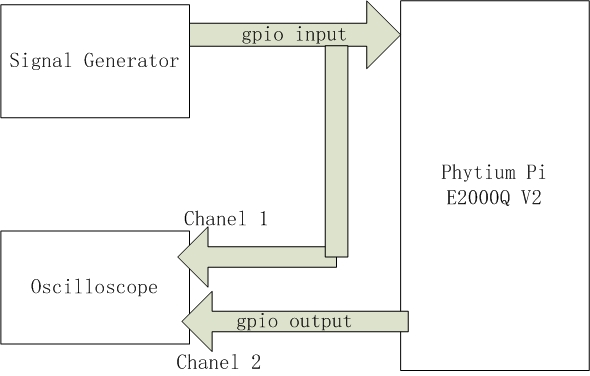
\includegraphics[width=0.85\columnwidth]{evaluation.jpg}
    \caption{System architecture.}
    \label{fig:oscilloscope}
\end{figure}


\textbf{Screenshot Analysis:}  
Waveform screenshots are provided, with markers indicating the shortest and longest response times of the output signal relative to the input trigger. The jitter is calculated as the difference between the maximum and minimum response times:  

\[
Jitter = T\_{max} - T\_{min}
\]


Here, the left edge of the persistence trace corresponds to the shortest response, while the right edge corresponds to the longest response.  

\begin{figure}[h]
  \centering
  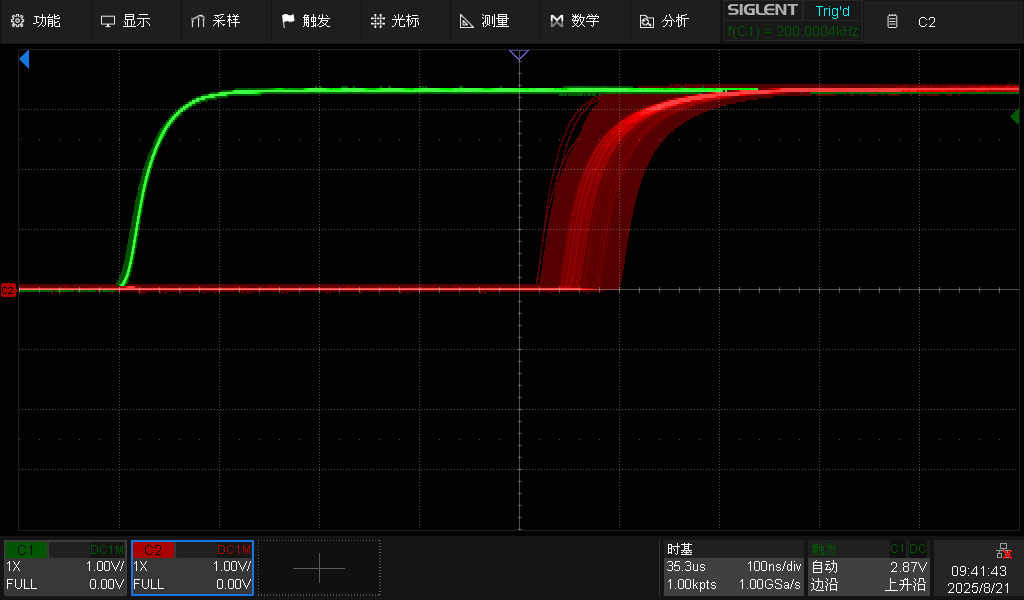
\includegraphics[width=0.8\linewidth]{oscilloscope.png}
  \caption{Oscilloscope persistence waveform showing shortest (left) and longest (right) GPIO response times (isolator)}
  \label{fig:jitter_waveform}
\end{figure}

\subsection{Experimental Results}
In a 24-hour continuous test, the system with isolator technology achieved, as show in Figure~\ref{fig:jitter_waveform}:
\begin{itemize}
    \item Maximum response latency: 500 ns
    \item Minimum response latency: 410 ns
    \item Jitter: 90 ns
\end{itemize}


By contrast, in a 24-hour continuous test,  PREEMPT-RT Linux system can only achieve maximum response latency:
110us.

\begin{figure}[h]
  \centering
  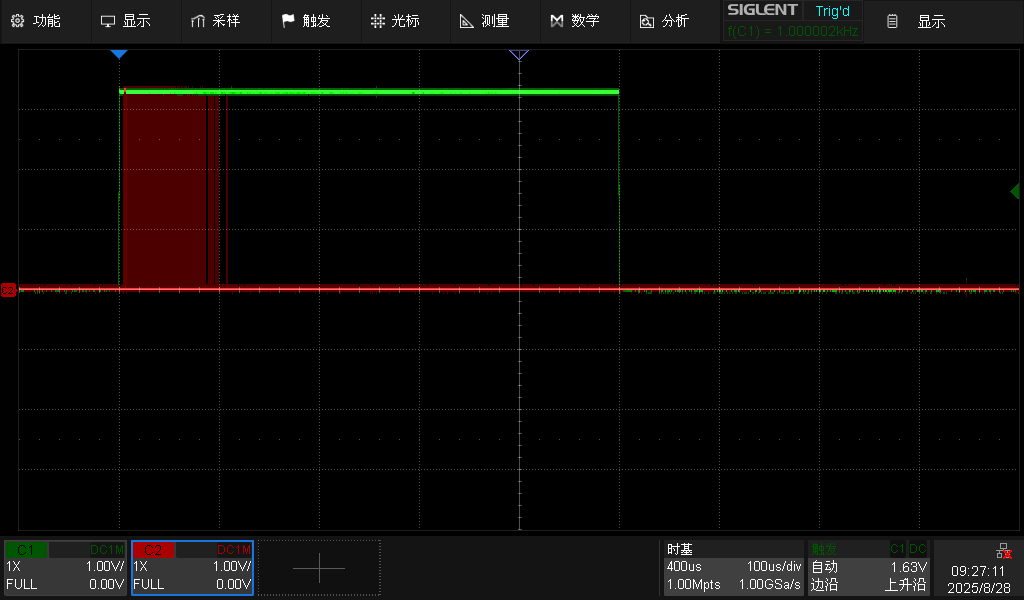
\includegraphics[width=0.8\linewidth]{oscilloscope2.png}
  \caption{Oscilloscope persistence waveform showing shortest (left) and longest (right) GPIO response times (PREEMPT-RT Linux)}
  \label{fig:jitter_waveform1}
\end{figure}


In addition to the external signal generator driven experiment, we implemented a counter-based GPIO toggling program. In this setup, the output signal is generated periodically by continuously reading the CPU timestamp counter (\texttt{CNTVCT\_EL0}) and flipping the GPIO at predefined intervals, eliminating the need for an external signal source.

The long-term experiment was conducted for 24 hours under both CPU-isolated and non-isolated environments. The results are summarized in Table~\ref{tab:counter_toggle}, showing that the isolator achieves sub-microsecond determinism, while non-isolated real-time Linux suffers from significantly larger latency
as shown in Figure~\ref{fig:jitter_waveform3} and Figure~\ref{fig:jitter_waveform4} .

\begin{figure}[h]
  \centering
  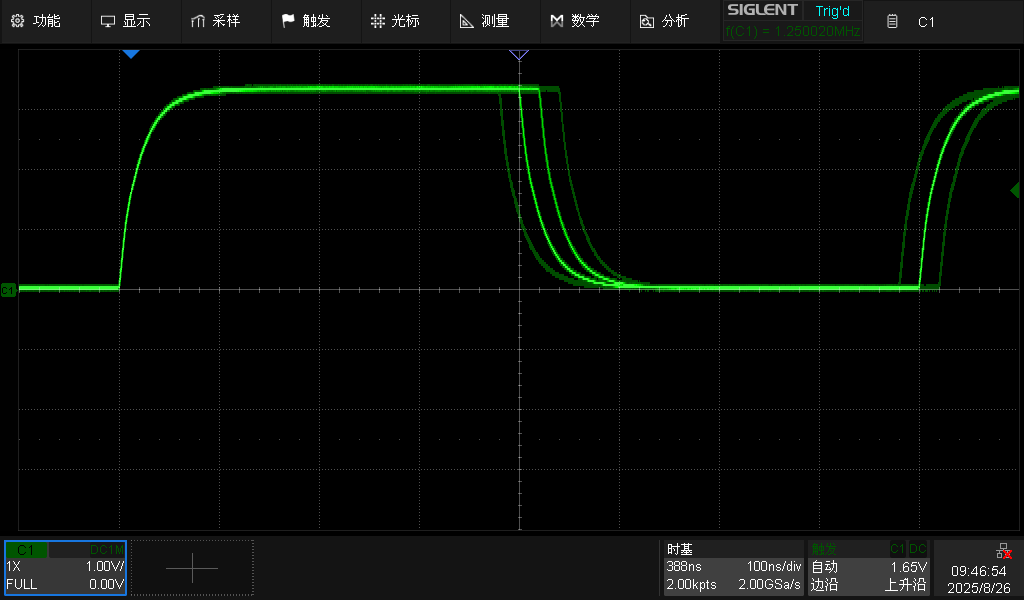
\includegraphics[width=0.8\linewidth]{oscilloscope3.png}
  \caption{Oscilloscope maximum deviation (isolator)}
  \label{fig:jitter_waveform3}
\end{figure}

\begin{figure}[h]
  \centering
  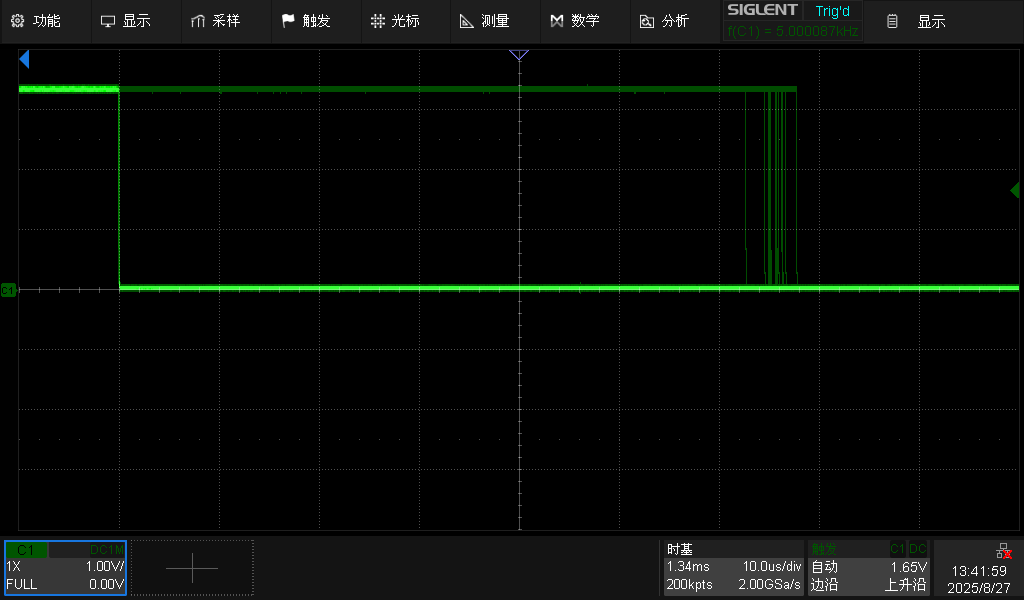
\includegraphics[width=0.8\linewidth]{oscilloscope4.png}
  \caption{Oscilloscope maximum deviation (PREEMPT-RT Linux)}
  \label{fig:jitter_waveform4}
\end{figure}

\begin{table}[h]
\centering
\caption{Counter-based GPIO toggling experiment results over 24 hours}
\label{tab:counter_toggle}
\begin{tabular}{lccc}
\hline
\textbf{Configuration} & \textbf{Period} & \textbf{Maximum Latency} & \textbf{Duration} \\
\hline
With Isolator & 800~ns & 60~ns & 24~h \\
Without Isolator & 200~\(\mu\)s & 680~\(\mu\)s & 24~h \\
\hline
\end{tabular}
\end{table}

The experiments demonstrate that using the isolator significantly improves GPIO signal determinism on the Phytium Pi development board. When triggered by an external signal generator, the isolator-enabled system achieves sub-microsecond maximum latency and minimal jitter (90 ns), as visualized through the oscilloscope persistence mode. In contrast, a standard PREEMPT-RT Linux system exhibits much higher latency (up to 110 µs). The counter-based GPIO toggling test over 24 hours further confirms that CPU isolation with the isolator ensures stable, predictable timing, whereas non-isolated real-time Linux shows large and inconsistent latencies. Overall, the isolator provides robust deterministic execution for time-critical GPIO operations.

\section{Summary}
This paper introduced a kernel-level isolation framework that enables deterministic sub-microsecond
execution on Linux by eliminating involuntary interruptions on dedicated cores. The proposed design
suppresses periodic tick timers, defers real-time bandwidth enforcement, and replaces asynchronous
inter-processor interrupts with shared-memory coordination. Through the Isolator API, applications
retain explicit control over when and how deferred maintenance tasks are executed, preserving both
determinism and system correctness.  

Evaluation on the Phytium Pi platform demonstrates the effectiveness of this approach. Under
isolator-enabled operation, GPIO response latencies consistently remain below 500~ns with jitter as
low as 90~ns, compared to up to 110~µs latency observed on PREEMPT-RT Linux. A long-term
counter-based GPIO toggling experiment further validated that the isolator achieves stable,
sub-microsecond determinism over 24 hours, while non-isolated real-time Linux exhibited latency
fluctuations in the hundreds of microseconds.  

Together, these results highlight that interrupt isolation and cooperative tick management provide a
lightweight yet powerful strategy for achieving predictable performance on general-purpose
operating systems. The framework enables strong temporal isolation and low-jitter execution,
making it well suited for latency-critical scenarios such as packet processing, edge computing, and
real-time control in embedded systems.

\newpage
% \printbibliography 
\bibliographystyle{flairs} 
\bibliography{references.bib}


% \clearpage
\onecolumn
\section*{Appendix}
This section includes additional sample snapshots of malicious videos.
% \begin{figure}[htp]
%     \centering
%     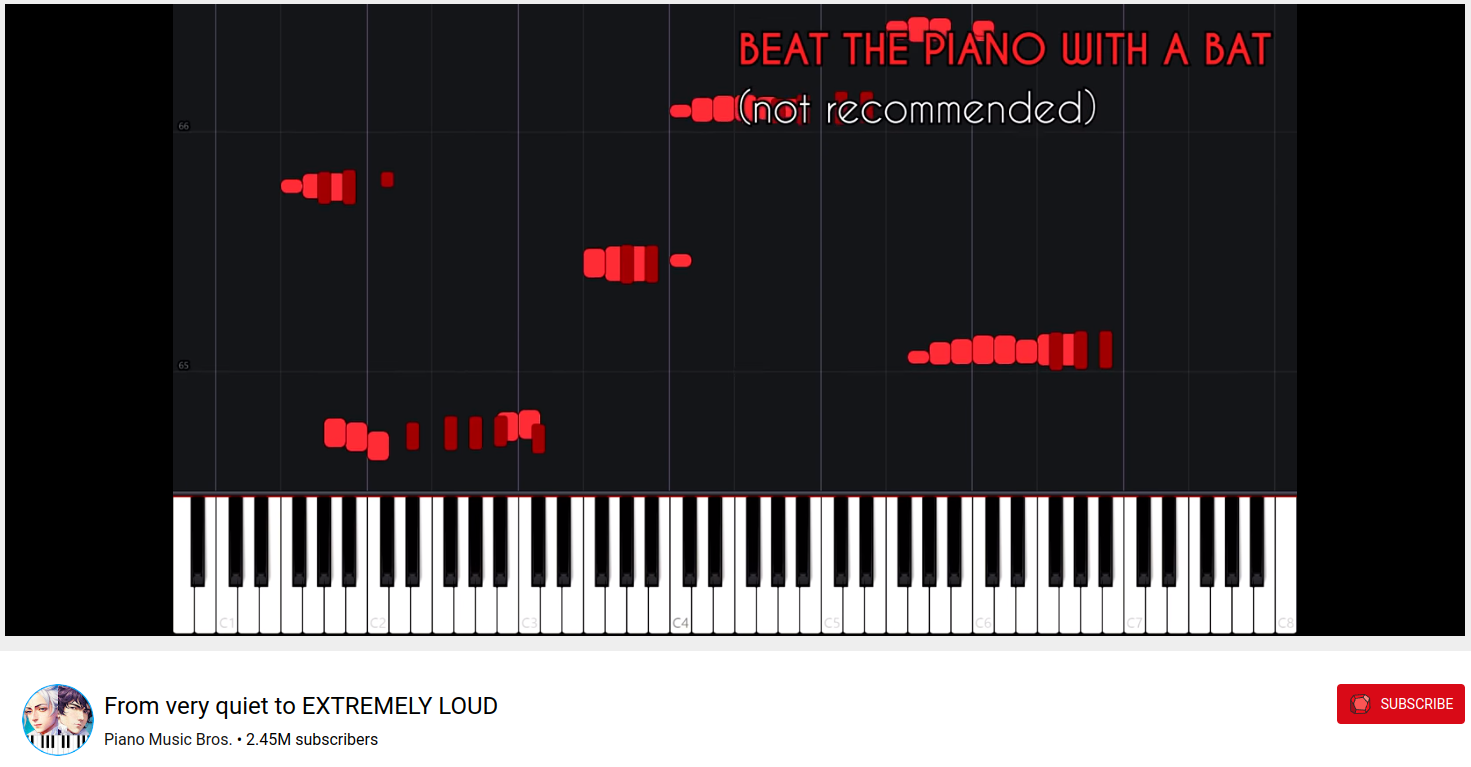
\includegraphics[width=0.6\columnwidth]{figures/malicious_audio.png}
%     \caption{A sample video which includes fast and loud piano notes. Usually in such videos, there is high tempo, no rhythm and varying pitches. The video also includes bright and striking hues, and also suggests a violent action of "hitting the piano with a bat"!}
%     \label{fig:ytkpiano}
% \end{figure}




\begin{figure}[!htb]
  \centering

  \begin{subfigure}{0.45\textwidth}
    \centering
    
\includegraphics[width=\textwidth]{figures/malicious7.png}
    \caption{}
    \label{fig:image_a}
  \end{subfigure}
  \hfill
  \begin{subfigure}{0.45\textwidth}
    \centering
    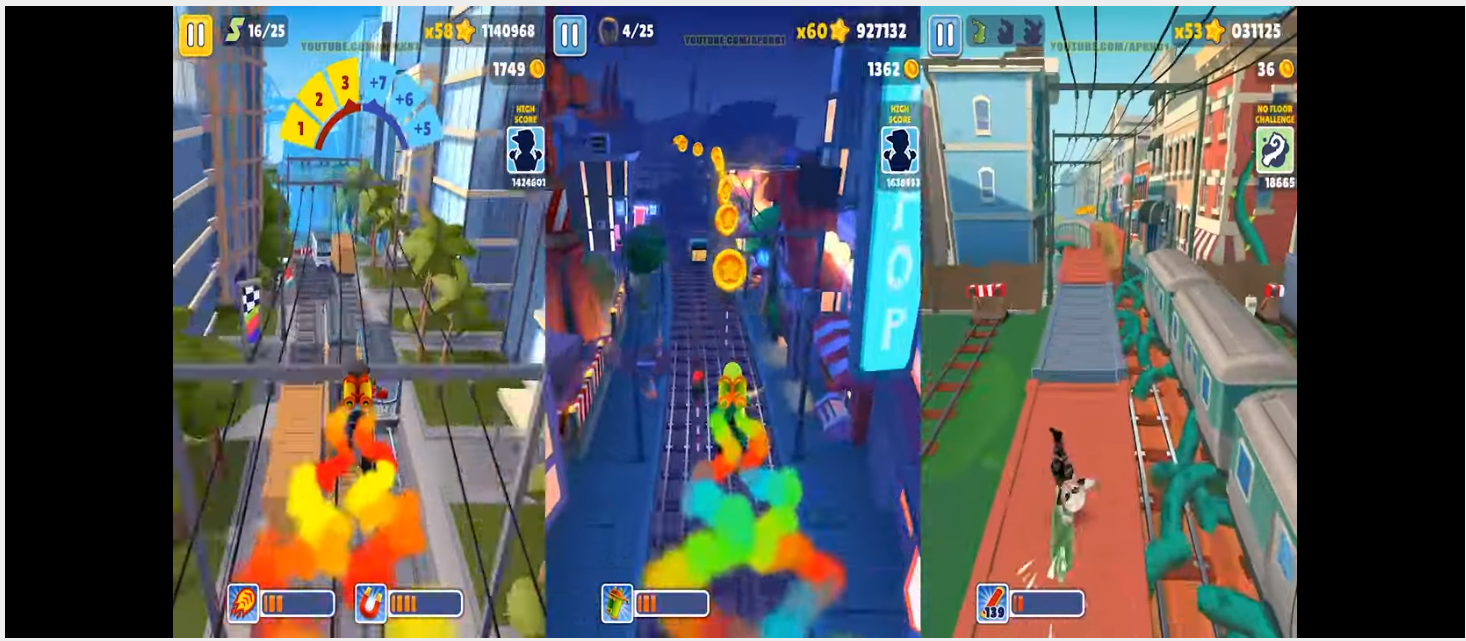
\includegraphics[width=\textwidth]{figures/malicious8.png}
    \caption{}
    \label{fig:image_b}
  \end{subfigure}

  \caption{a) shows a gameplay having striking colors which includes 2 different animations in 2 halves of the screen. b) shows a sample gameplay video for the Subway Surfer game displayed in a split-screen layout.}
  \label{fig:group_of_images}
\end{figure}

\begin{figure}[!htb]
  \centering

  \begin{subfigure}{0.45\textwidth}
    \centering
    
\includegraphics[width=0.8\textwidth]{figures/malicious5.png}
    \caption{}
    \label{fig:image_disgust}
  \end{subfigure}
  \hfill
  \begin{subfigure}{0.45\textwidth}
    \centering
    
\includegraphics[width=\textwidth]{figures/malicious9.png}
    \caption{}
    \label{fig:image_angry}
  \end{subfigure}

  \caption{a) shows a disgusting and scary character b) shows a furious and frightening PacMan.}
  \label{fig:disgusting}
\end{figure}

\begin{figure*}[!h]
    \centering
    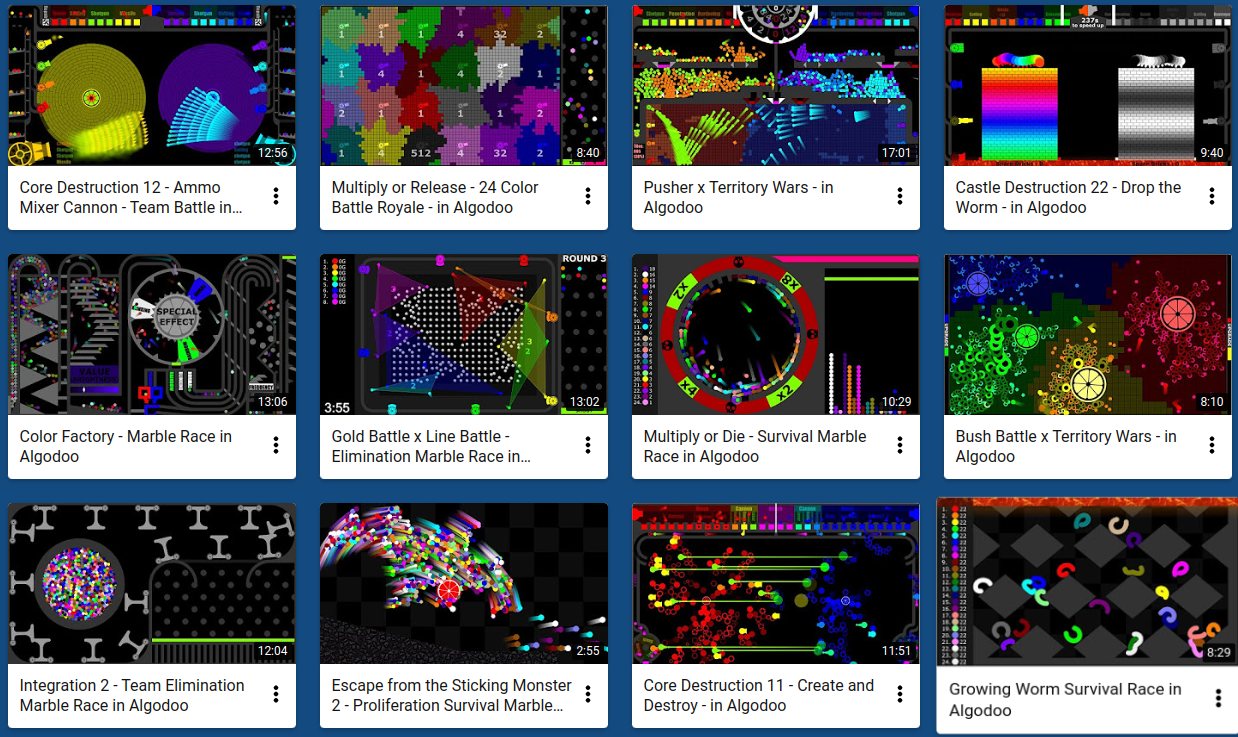
\includegraphics[width=0.8\textwidth]{figures/maliciou3.png}
    \caption{Videos of animations on YouTube Kids which include tiny fast-moving objects with bright colors.  The music soundtrack includes heavy metal and rock music.}  
    \label{fig:model}
\end{figure*}


% \begingroup
% \renewcommand{\arraystretch}{1.6}
% \begin{table}[h]
% \centering
% \begin{tabularx}{0.45\textwidth} { 
%   >{\raggedright\arraybackslash}X 
%   | >{\centering\arraybackslash}X 
%   | >{\centering\arraybackslash}X 
%   | >{\centering\arraybackslash}X
%   | >{\centering\arraybackslash}X 
%   | >{\centering\arraybackslash}X}
 
%  \textbf{Model} & \textbf{Layers} & \textbf{Patch Size} & \textbf{MLP Dim} & \textbf{Heads} & \textbf{Param} \\
%  \hline
%  \hline
%  ViT-B/16 & 12 & 16 & 3072 & 12 & 86M\\
%  ViT-B/32 & 12 & 32 & 3072 & 12 & 86M\\
%  % ViT-L/14 & 24 & 1024 & 4096 & 16 & 307M\\
% \end{tabularx}
% \caption{Comparison of CLIP base models.}
% \label{table:modelcomp}
% \end{table}
% \endgroup

\end{document}
